\documentclass{beamer}
\usepackage{setspace}
\usepackage{bm,color,float,epstopdf,amsthm,epstopdf}
\usepackage{multirow,tikz}
\newcommand{\fttheory}[1]{\fcolorbox{blue}{blue}{\color{white}\textbf{#1}\hspace{\textwidth}}}
\newcommand{\ftexampl}[1]{\fcolorbox{orange}{orange}{\color{black}\textbf{#1}\hspace{\textwidth}}}
\newcommand{\ftdata}[1]{\fcolorbox{violet}{violet}{\color{white}\textbf{#1}\hspace{\textwidth}}}
\newcommand{\ftheader}[1]{\fcolorbox{lightgray}{lightgray}{\color{black}\textbf{#1}\hspace{\textwidth}}}
\newcommand{\ftvocab}[1]{\fcolorbox{cyan}{cyan}{\color{black}\textbf{#1}\hspace{\textwidth}}}
\newcommand{\usd}{\text{ {\scriptsize USD}}}
\newcommand{\eur}{\text{ {\scriptsize EUR}}}
\newcommand{\aud}{\text{ {\scriptsize AUD}}}
\newcommand{\mxn}{\text{ {\scriptsize MXN}}}
\newcommand{\musd}{\text{ m {\scriptsize USD}}}
\newcommand{\meur}{\text{ m {\scriptsize EUR}}}
\newcommand{\maud}{\text{ m {\scriptsize AUD}}}

\renewcommand{\arraystretch}{1.5}
\begin{document}
%TODO: write a motivation slide
% Option Basics
\begin{frame}{\ftvocab{Option Basics}}
	\begin{itemize}
		\item An \textit{option} is a contract that gives its owner the \underline{right} (but not the \underline{obligation}) to buy or sell an asset at a pre-specified price (called the \textit{stike price}) at some future date (called \textit{expiration})
	\item a \textit{call option} gives the owner the \underline{right} to \underline{buy} the asset
	\item a \textit{put option} gives the owner the \underline{right} to \underline{sell} the asset 
	\item (the owner of a \textit{forward} is \underline{obligated} to buy the asset)
	\item Option buyers (a.k.a. owners) are \textit{long} 
	\item Option sellers (a.k.a. writers) are \textit{short}
	\end{itemize}
\end{frame}

% Understanding Option Contracts
\begin{frame}{\ftvocab{Option Basics}}
	\begin{itemize}
		\item When the owner buys or sells the asset at the strike price, she is \textit{exercising} the option. 
		\item There are two (more) kinds of options:
		\begin{itemize}
			\item American options allow their owners to exercise the option on any date up to and including the expiration date;
			\item European options allow their owners to exercise the option only on the expiration date. 
		\end{itemize}
		\item When you sell an option, you get paid for it. The market price of the option is also called the \textit{option premium}. 
		\item More vocabulary: an option is said to be
		\begin{itemize}
			\item \textbf{in-the-money} if the payoff from exercising an option immediately is positive;
			\item \textbf{at-the-money} if the payoff from exercising an option immediately is zero;
			\item \textbf{out-of-the-money} if the payoff from exercising an option immediately is negative;
		\end{itemize}
		\item The terms deep-in-the-money are commonly used deep-out-of-the-money.
	\end{itemize}
\end{frame}

% Long Position in a Call
\begin{frame}{\fttheory{Long Position in a Call}}
	Let $S$ denote the stock price at expiration, $K$ the strike price, and $C$ the value of the call option. The value of a \textbf{long position} in the \textbf{call option} at expiration is 
	\begin{equation}
		\text{Value of Long Call}=C=\max\{S-K,0\}. 
	\end{equation}
	\begin{figure}[H]
		\begin{center}
			
\includegraphics[scale=.4]{longcall}
		\end{center}
	$K=20$
	\end{figure}
\end{frame}

\begin{frame}{\ftexampl{Examples: Long Call}}
	\input{payoff_NKE_long_call}
\end{frame}

\begin{frame}{\ftexampl{Examples: Long Call}}
	\noindent On 2020-03-31, MSFT traded for 162.01 USD. Suppose you were long a 150.95 USD call that expired on 2020-03-31. Was the option in, at, or out-of-the-money? Was the option exercised? What was your payoff at expiration?

\vspace{9pt} 

\textbf{Solution.}The option was in-the-money, so it was exericed.Your payoff was 6.76 USD.
\end{frame}

% Long Position in a Put
\begin{frame}{\fttheory{Long Position in a Put}}
Let $S$ denote the stock price at expiration, $K$ the strike price, and $P$ the value of the put option. The value of a \textbf{long position} in the \textbf{put option} at expiration is 
\begin{equation}
\text{Value of Long Put}=P=\max\{K-S,0\}. 
\end{equation}
\begin{figure}[H]
	\begin{center}
		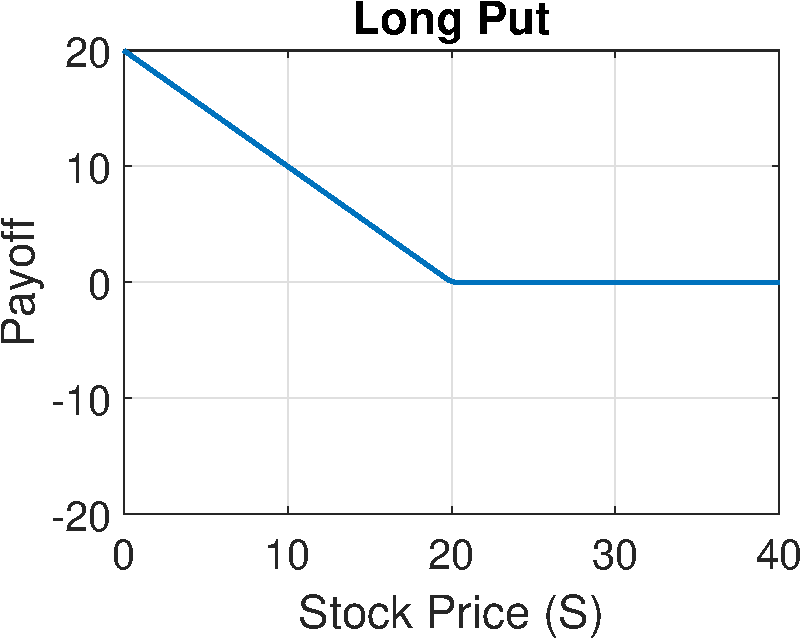
\includegraphics[scale=.4]{longput}
	\end{center}
	$K=20$
\end{figure}
\end{frame}

\begin{frame}{\ftexampl{Examples: Long Put}}
	\input{payoff_NKE_long_put}
\end{frame}

\begin{frame}{\ftexampl{Examples: Long Put}}
	\noindent On 2020-03-31, MSFT traded for 162.01 USD. Suppose you were long a 150.95 USD put that expired on 2020-03-31. Was the option in, at, or out-of-the-money? Was the option exercised? What was your payoff at expiration?

\vspace{9pt} 

\textbf{Solution.}The option was out-of-the-money, so it was not exercised. Your payoff was 0 USD.
\end{frame}

% Short Position in a Call
\begin{frame}{\fttheory{Short Position in a Call}}
Let $S$ denote the stock price at expiration, $K$ the strike price, and $C$ the value of the call option. The value of a \textbf{short position} in the \textbf{call option} at expiration is 
\begin{equation}
\text{Value of Short Call}=-C=-\max\{S-K,0\}. 
\end{equation}
\begin{figure}[H]
	\begin{center}
		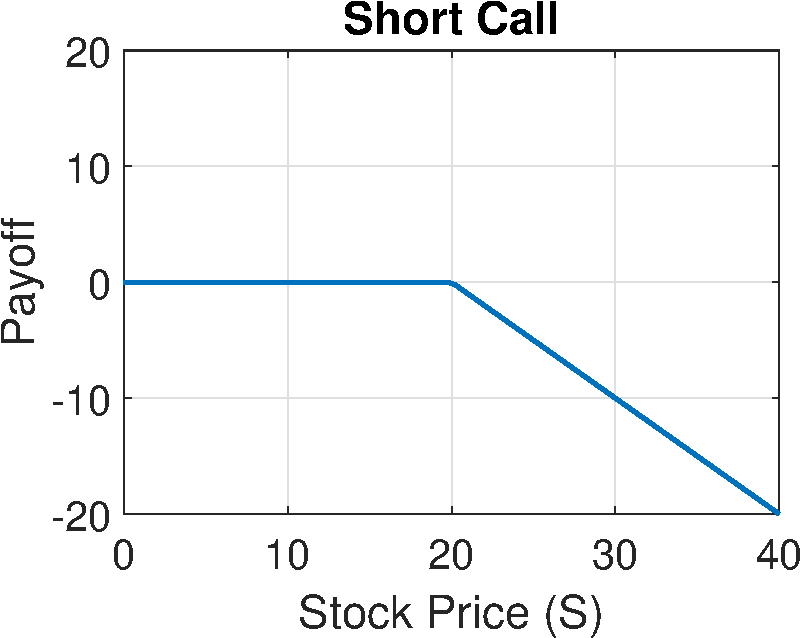
\includegraphics[scale=.4]{shortcall}
	\end{center}
	$K=20$
\end{figure}
\end{frame}

\begin{frame}{\ftexampl{Examples: Short Call}}
	\input{payoff_NKE_short_call}
\end{frame}

\begin{frame}{\ftexampl{Examples: Short Call}}
	\input{payoff_MSFT_short_call}
\end{frame}

% Short Position in a Put
\begin{frame}{\fttheory{Short Position in a Put}}
Let $S$ denote the stock price at expiration, $K$ the strike price, and $P$ the value of the put option. The value of a \textbf{short position} in the \textbf{put option} at expiration is 
\begin{equation}
\text{Value of Short Put}=-P=-\max\{K-S,0\}. 
\end{equation}
\begin{figure}[H]
	\begin{center}
		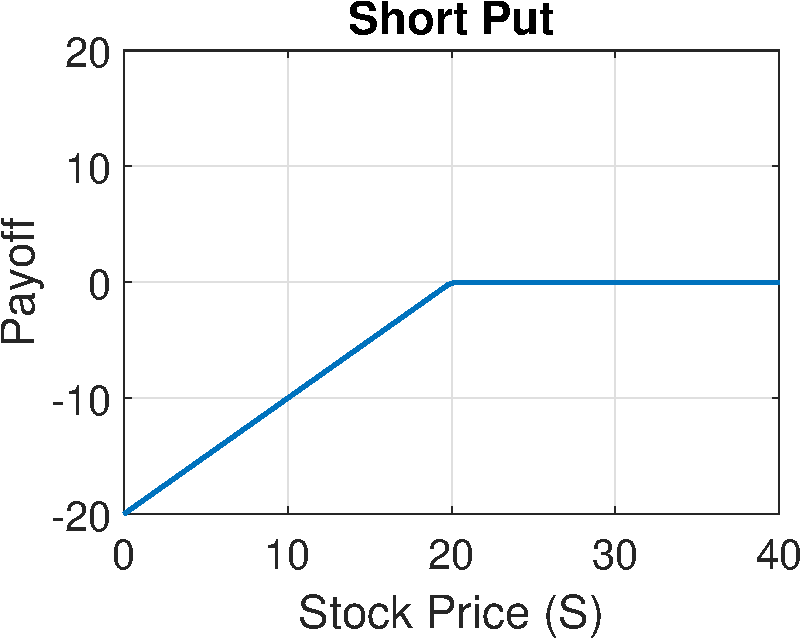
\includegraphics[scale=.4]{shortput}
	\end{center}
	$K=20$
\end{figure}
\end{frame}

\begin{frame}{\ftexampl{Examples: Short Put}}
	\input{payoff_NKE_short_put}
\end{frame}

\begin{frame}{\ftexampl{Examples: Short Put}}
	\input{payoff_MSFT_short_put}
\end{frame}

% The Covered Call
\begin{frame}{\fttheory{The Covered Call}}
Let $S$ denote the stock price at expiration, $K$ the strike price, and $C$ the value of the call option. A \textbf{covered call} is \textbf{long} the \textbf{underlying} and \textbf{short} a \textbf{call}. Its value at expiration is
\begin{equation}
\text{Value of Covered Call}=S-C(S;K)=\min\{S,K\}
\end{equation}
\begin{figure}[H]
	\begin{center}
		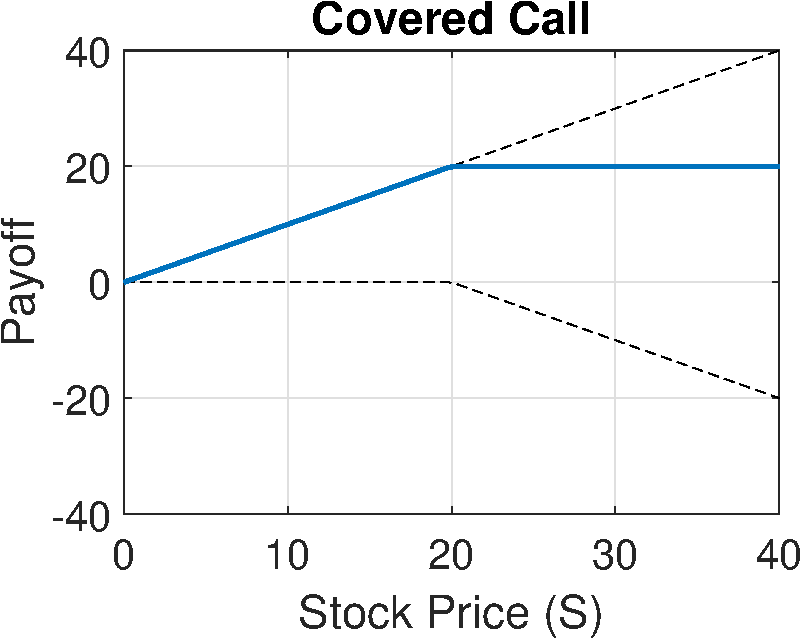
\includegraphics[scale=.4]{coveredcall}
	\end{center}
	$K=20$
\end{figure}
\end{frame}

% The Married Put
\begin{frame}{\fttheory{The Married Put}}
Let $S$ denote the stock price at expiration, $K$ the strike price, and $P$ the value of the put option. A \textbf{married put} is \textbf{long} the \textbf{underlying} and \textbf{long} a \textbf{put}. Its value at expiration is
\begin{equation}
\text{Value of Married Put}=S+P(S;K)=\max\{K,S\}.  
\end{equation}
\begin{figure}[H]
	\begin{center}
		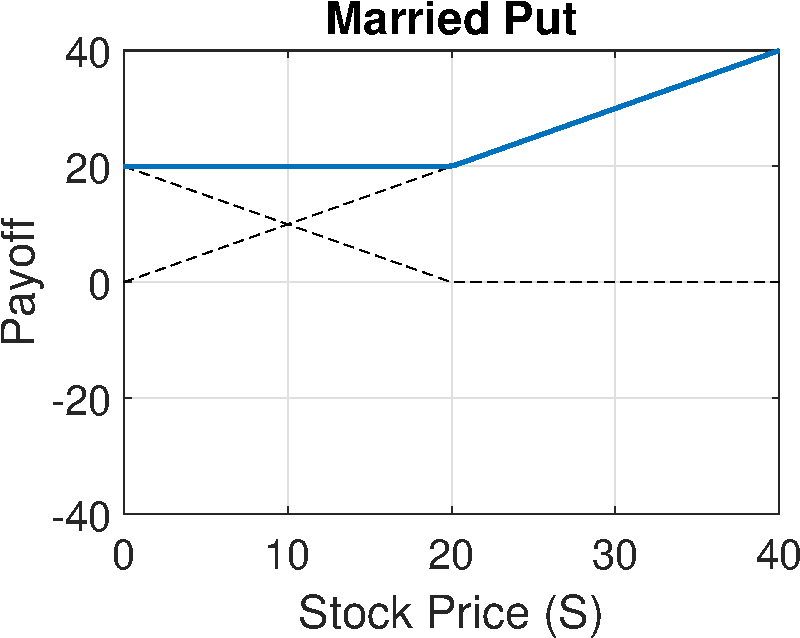
\includegraphics[scale=.4]{marriedput}
	\end{center}
	$K=20$
\end{figure}
\end{frame}

% The Structured Product
\begin{frame}{\fttheory{The Structured Product}}
A structured product is \textbf{long} the \textbf{risk-free asset} and \textbf{long} a \textbf{call}. Its value at expiration is
\begin{equation}
\text{Value of Structured Product}=K+C(S;K)=\max\{S,K\}.  
\end{equation}
\begin{figure}[H]
	\begin{center}
		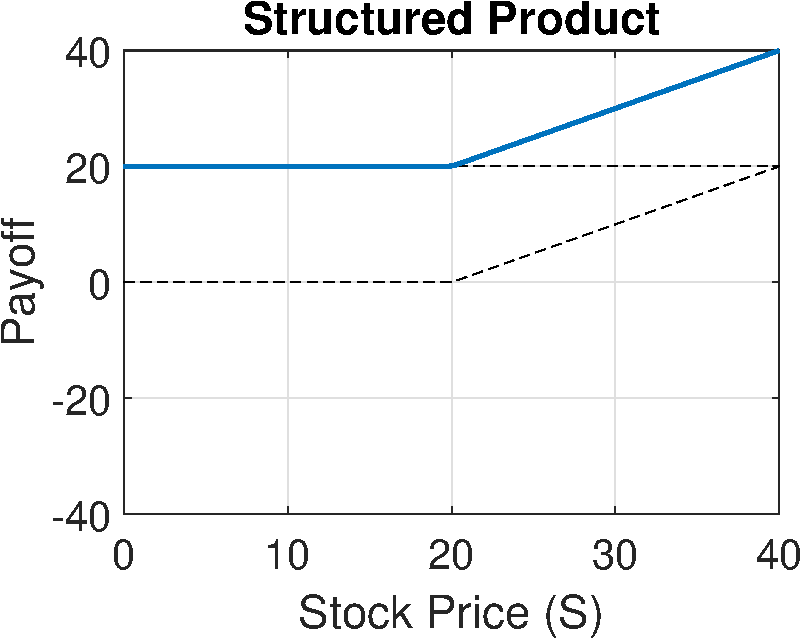
\includegraphics[scale=.4]{structuredproduct}
	\end{center}
	$K=20$
\end{figure}
\end{frame}

% Put-Call Parity
\begin{frame}{\fttheory{Put-Call Parity}}
\begin{itemize}
\item The Structured Product has same payoff as the Married Put
\item Two securities with same cash flows must have the same price
\item \textbf{Put-Call Parity} says that
\begin{equation}
	\overbrace{S_{0}+P_{0}}^{\text{Married Put}}=\overbrace{PV(K)+C_{0}}^{\text{Structured Product}}
\end{equation}
		where $S_{0}$ is the spot price of the stock, $P_{0}$ is the put premium, $C_{0}$ is the call premium, and $PV(K)$ is the price of a zero-coupon bond that pays $K$ at expiration
\item Put-call parity gives the price of a call in terms of the price of a put, the underlying stock, and a zero-coupon bond. 
\end{itemize}
\end{frame}

\iffalse
% Equity as a Call Option
\begin{frame}{\fttheory{Equity as a Call Option}}
Consider a firm with 10m USD in debt. It will only operate for one year. At the end of the year, its assets maybe worth anywhere from 0m USD to 40m USD. What's the payoff to \textbf{equityholders}?
\begin{equation}
	E=\max\{A-K,0\}\overset{!}{=}\max\{A-10\text{m USD},0\}. 
\end{equation}
\begin{figure}[H]
	\begin{center}
		
\includegraphics[scale=.4]{equity}
	\end{center}
\end{figure}
\end{frame}

% Debt as a Covered Call
\begin{frame}{\fttheory{Debt as a Covered Call}}
Consider a firm with 10m USD in debt. It will only operate for one year. At the end of the year, its assets maybe worth anywhere from 0m USD to 40m USD. What's the payoff to \textbf{debtholders}?
\begin{equation}
	D=\min\{A,K\}\overset{!}{=}\min\{A,10\text{m USD}\}. 
\end{equation}
\begin{figure}[H]
	\begin{center}
		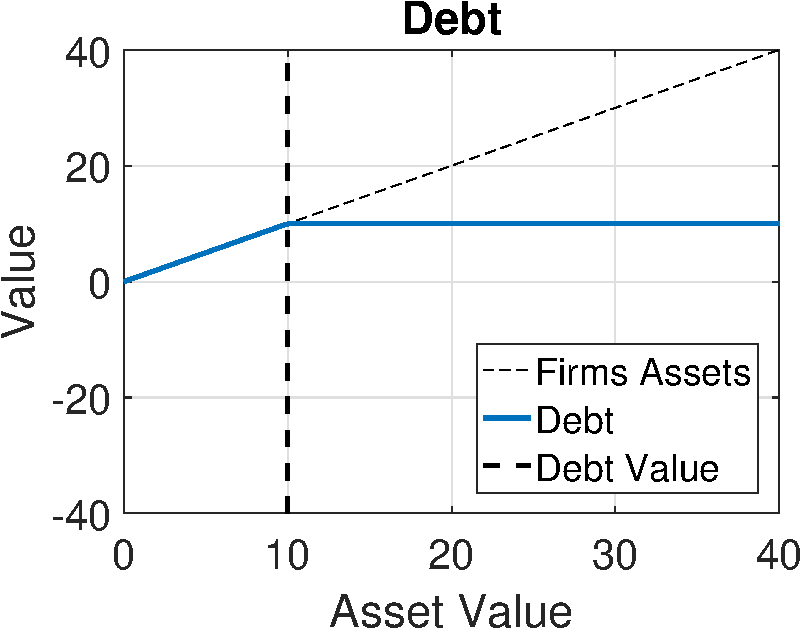
\includegraphics[scale=.4]{debt}
	\end{center}
\end{figure}
\end{frame}

% The Total Payoff
\begin{frame}{\fttheory{The Total Payoff}}
Now what's the \textbf{total payoff}?
\begin{equation}
E+D=\max\{A-K,0\}+\min\{A,K\}=A
\end{equation}
\begin{figure}[H]
	\begin{center}
		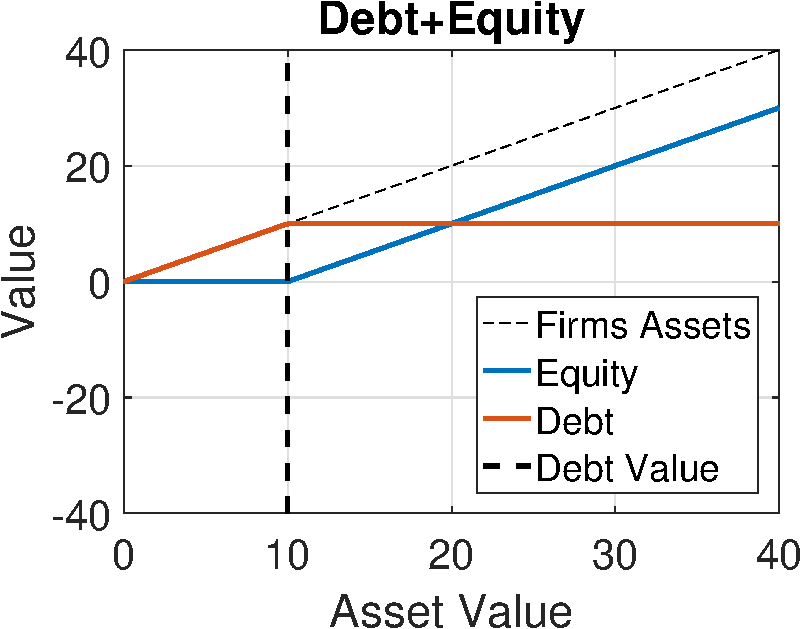
\includegraphics[scale=.4]{debtequity}
	\end{center}
\end{figure}
\end{frame}
\fi

\end{document}
